\newgeometry{a4paper, top=5mm, left=25mm, right=25mm, bottom=30mm,headsep=5mm, footskip=12mm}
\begin{titlepage}
\begin{minipage}[t]{0.25\textwidth}\end{minipage}\hfill
\begin{minipage}[t]{0.7\textwidth}
\includegraphics[width=\textwidth]{images/rwth_ltt_de_rgb}\end{minipage}
	\begin{center}
	    Diese Arbeit wurde vorgelegt am Lehrstuhl für Technische Thermodynamik
	\end{center}

\vspace{5em}   %LTT-Vorlage: 11em
	\begin{center}
	    {\fontsize{24}{26} \selectfont \textbf{Application and Assessment of \\ Simplified Process Design Methods for Generating Life Cycle Assessment Databases for Chemicals \par}}
	\end{center}
	
		\vspace{4em}
		
	{\fontsize{18}{22} \selectfont Projektarbeit}\\
		\vspace{2em}\\
		
	{\fontsize{14}{18} \selectfont Von}
	
	{\fontsize{14}{18} \selectfont Valentin Dinges und Matthias Ellinger}\\\\
		\vspace{7em} 
		

{\fontsize{14}{18} \selectfont Prüfer: Professor Dr.-Ing. André Bardow }

{\fontsize{14}{18} \selectfont Betreuer:  Raoul Meys, M. Sc.}
		\vspace{3em} 

\hfill\begin{minipage}{0.35\textwidth}{\fontsize{14}{16} \selectfont Aachen, den 27.03.2020}
\end{minipage}
\restoregeometry
\end{titlepage}

\begin{titlepage}


%%Leere Seite
%\newpage\thispagestyle{empty}\hspace{1em}\newpage
% \thispagestyle{plain}
% \newpage\thispagestyle{empty}\hspace{1em}\newpage
% \thispagestyle{plain}
% Erklaerung


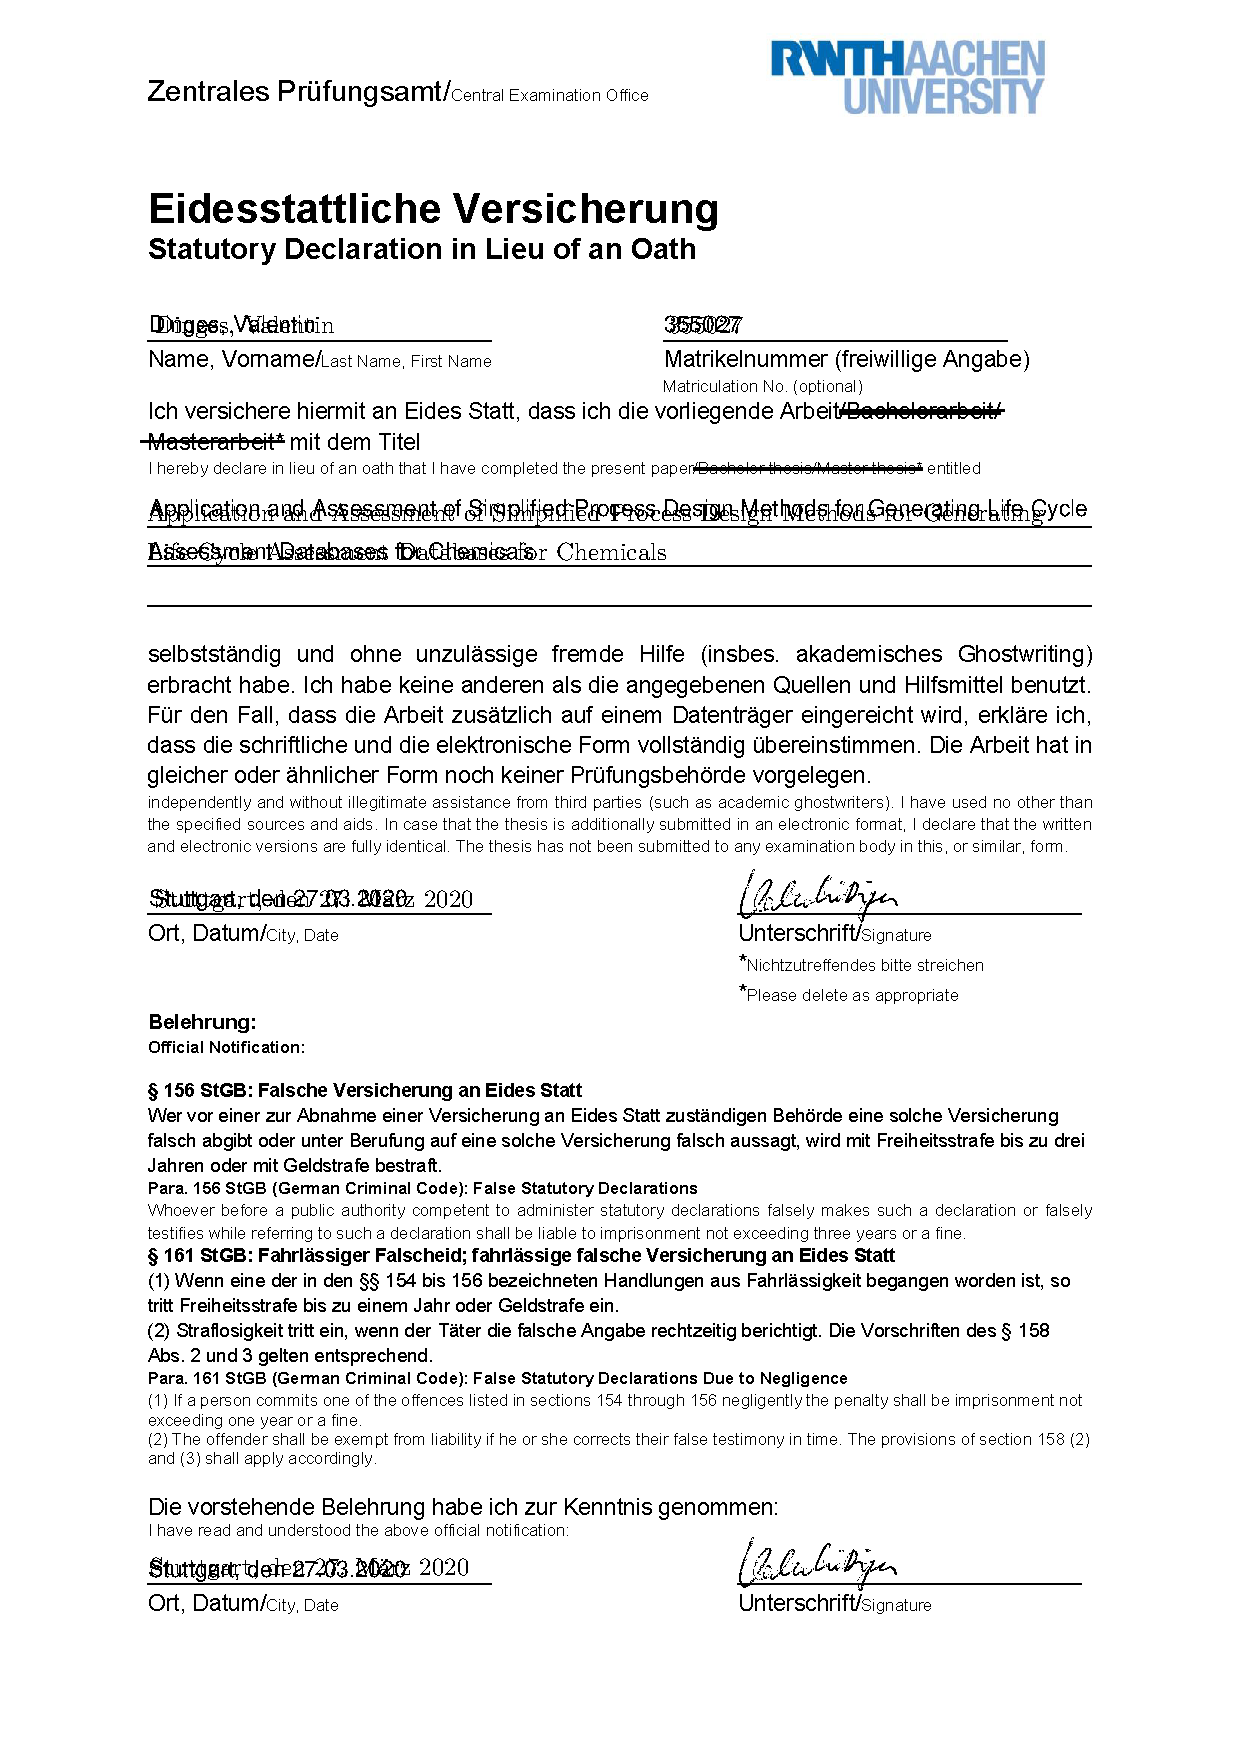
\includepdf{images/EidesstattlicheVersicherung_Dinges.pdf}
\cleardoublepage
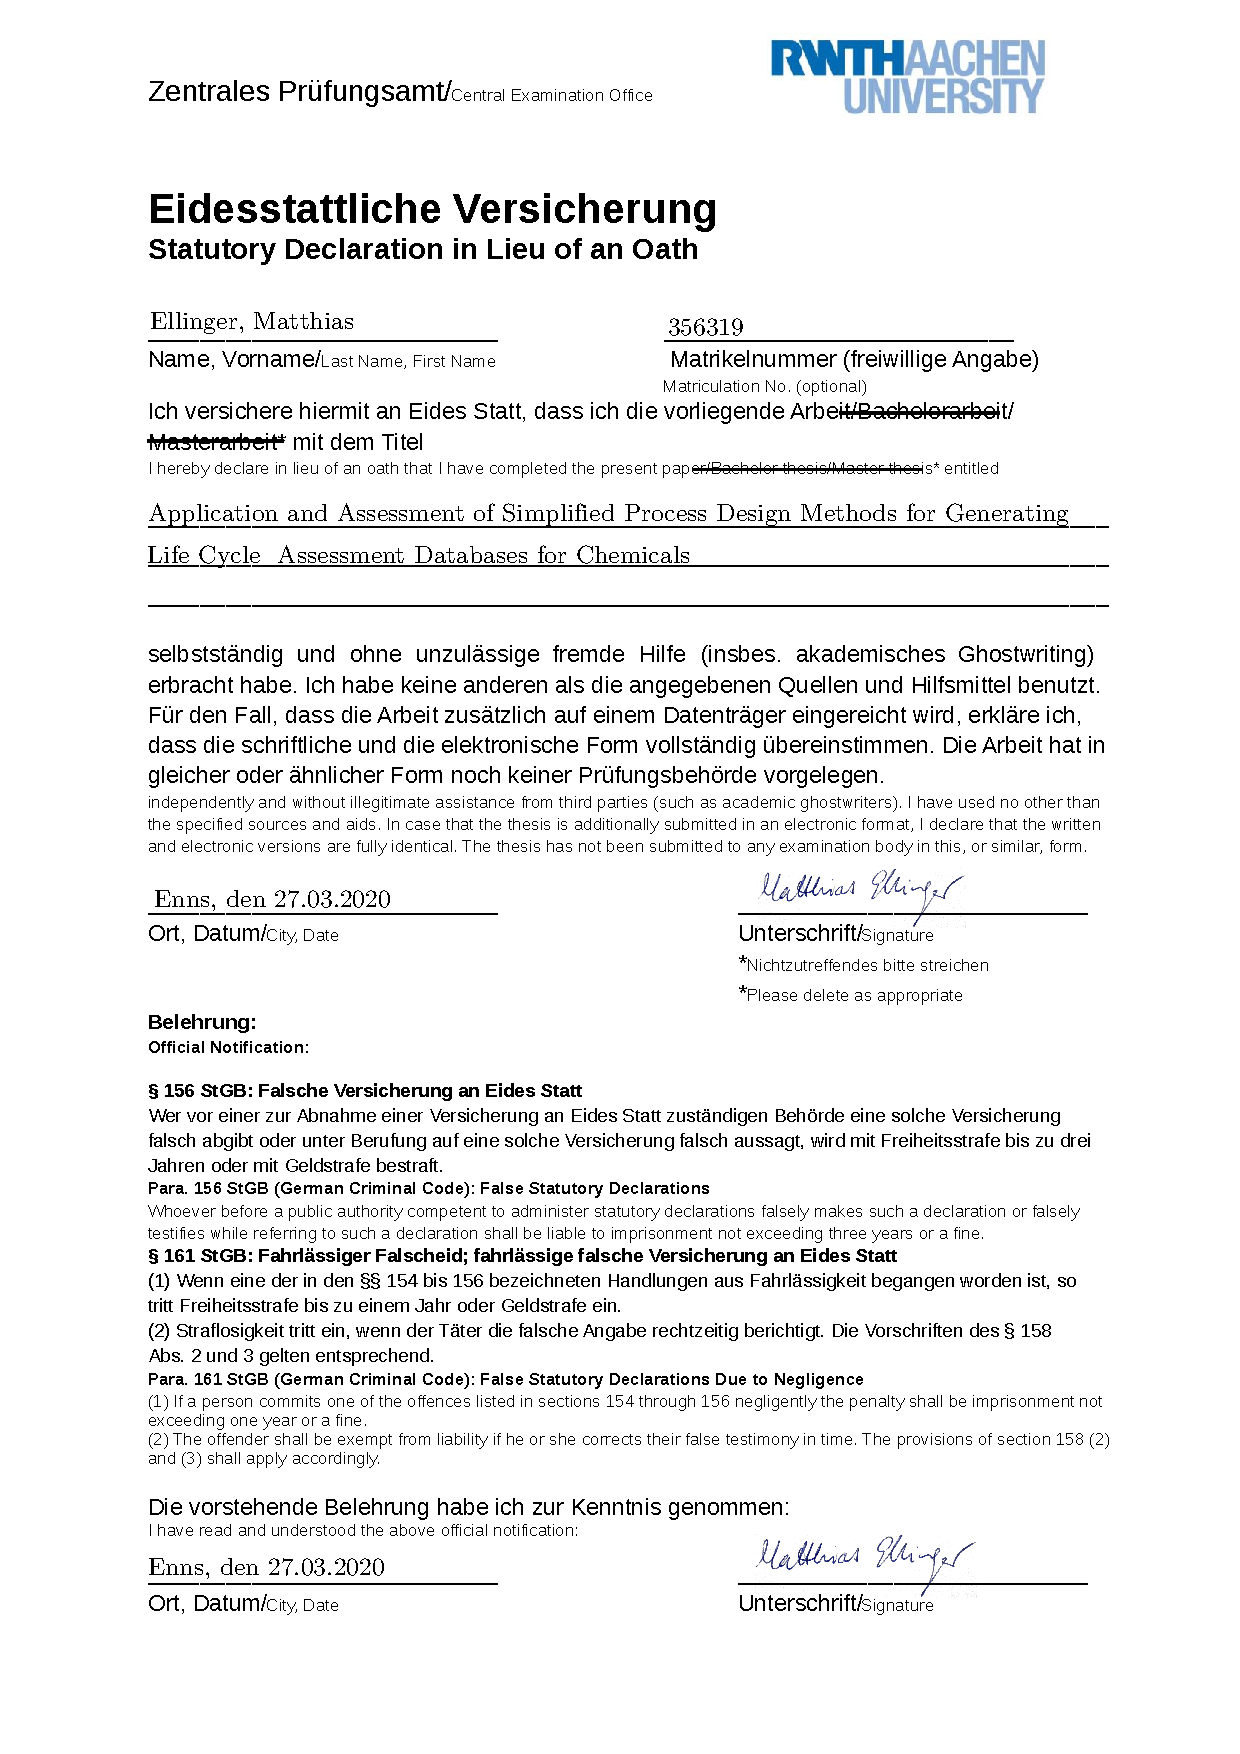
\includepdf{images/EidesstattlicheVersicherung_Ellinger.pdf}


\end{titlepage}
\cleardoublepage

%Leere Seite
%\newpage\thispagestyle{empty}\hspace{1em}\newpage


%\addtolength{\cftparskip}{6pt} 
%\addtolength{\cftparskip}{5pt} 

%\addtocontents{toc}{\vspace{-5ex}}
